\documentclass[10pt,twocolumn,letterpaper]{article}

\usepackage{cvpr}
%% This file contains a number of tweaks that are typically applied to the main document.
%% They are not enabled by default, but can be enabled by uncommenting the relevant lines.


%%
%% Official support for 2-column teaser figure
%%
\usepackage{cuted} %< for strip environment

%%
%% For auto-referencing of figures (see fig/teaser.tex and \label{} therein) 
%%
\usepackage{currfile} %< for \currfilebase macro

%%
%% caption and (global) spacing overrides
%%
\usepackage{caption} %< for "\captionof" commands (teaser)
% \setlength{\abovecaptionskip}{.5em} % space above caption
% \setlength{\belowcaptionskip}{1em} % space below caption

%%
%% Inline annotations; for predefined colors, refer to "dvipsnames" in the xcolor package:
%% https://tinyurl.com/overleaf-colors
%%
\newcommand{\red}[1]{{\color{red}#1}}
\newcommand{\todo}[1]{{\color{red}#1}}
\newcommand{\TODO}[1]{\textbf{\color{red}[TODO: #1]}}
%%
%% Disable for camera ready / submission by uncommenting these lines:
%%
% \renewcommand{\TODO}[1]{}
% \renewcommand{\todo}[1]{#1}

%%
%% Work harder in optimizing text layout. Typically shrinks text by 1/6 of page, enable
%% it at the very end of the writing process, when you are just above the page limit.
%%
% \usepackage{microtype}

%%
%% Fine-tune paragraph spacing.
%%
% \renewcommand{\paragraph}[1]{\vspace{.5em}\noindent\textbf{#1.}}

%%
%% Globally adjusts space between figure and caption.
%%
% \setlength{\abovecaptionskip}{.5em}

%%
%% Allows "the use of \paper to refer to the project name"
%% with automatic management of space at the end of the word.
%%
% \usepackage{xspace}
% \newcommand{\paper}{ProjectName\xspace}

%%
%% Commonly used math definitions.
%%
% \DeclareMathOperator*{\argmin}{arg\,min}
% \DeclareMathOperator*{\argmax}{arg\,max}

%%
%% Tighten underline.
%%
% \usepackage{soul}
% \setuldepth{foobar}

%%
%% Reconfigure paragraph (tweaks spacing)
%%


\definecolor{cvprblue}{rgb}{0.21,0.49,0.74}
\usepackage[breaklinks,colorlinks,allcolors=cvprblue]{hyperref}

\usepackage{amsmath,amssymb}
\usepackage{booktabs}
\usepackage{multirow}
\usepackage{tikz}
\usepackage{placeins}
\usetikzlibrary{positioning,arrows.meta}

\def\confName{BTP Report}
\def\confYear{2026}

\title{Deep Learning for Hyperspectral Image Super-Resolution:\\From Global Dynamic Attention to Spatially-Aware Spectral Sparsity}

\author{Hemanth Sai Machireddy\\
B.Tech in Artificial Intelligence and Data Science\\
Indian Institute of Information Technology (IIIT) Sri City\\
{\tt\small Roll No. S0230030389}
\and
Dr. Adduru U G Sankararao\\
Supervisor, IIIT Sri City\\
{\tt\small November 2026}}

\begin{document}
\maketitle

\clearpage
\onecolumn
\tableofcontents
\listoffigures
\listoftables
\clearpage
\twocolumn

\begin{abstract}
Hyperspectral image super-resolution (HSI-SR) must simultaneously recover fine spatial structure and preserve inter-band spectral consistency. This thesis investigates two complementary directions across a two-semester research progression: GEWDiff, a generative RWA-PCA-EDM diffusion framework, and SDANet, a reconstruction-oriented dynamic spectral attention architecture. The GEWDiff investigation is documented with its published WDC result and a verified 22.2K CFG guidance sweep; the unavailable 31K guidance-scale provenance is explicitly identified. The final SDANet contribution introduces Spatially-Aware Dynamic Sparsity (SADS), which assigns independent $2\times2$ regional sparsity budgets while retaining shared query, key, and value representations. Fine-gate, independent-upsampler, matched 66K, and fusion diagnostics are reported only within their verified protocols. The contribution is framed as an implementation and mechanism analysis on Chikusei, not as a claim of cross-dataset or universal superiority.
\end{abstract}

\section{Chapter 1: Introduction}
\label{sec:introduction}

\subsection{Background and Motivation}

Hyperspectral imaging records hundreds of narrow spectral bands for each spatial location. Unlike conventional RGB or multispectral imagery, a hyperspectral cube can distinguish materials, vegetation conditions, geological surfaces, and subtle spectral signatures. The benefit of high spectral resolution comes with a measurement trade-off: narrow-band sensors and practical hardware constraints often reduce spatial resolution. A low-resolution hyperspectral image may therefore contain enough spectral information to characterize materials but insufficient spatial detail to localize them precisely.

This trade-off is important in agriculture, mineral mapping, environmental monitoring, urban analysis, and remote-sensing applications. For example, the land cover at a pixel boundary may contain mixed materials, yet independent band-wise reconstruction can distort the spectral signature or remove edge structure. Hyperspectral image super-resolution (HSI-SR) seeks to estimate a high-resolution cube from one or more lower-resolution observations. The task differs from ordinary RGB super-resolution because reconstruction errors are coupled across spectral bands and must be assessed by both spatial similarity and spectral angle.

A central research challenge is to preserve three kinds of consistency. Spatial fidelity requires edges and small structures to be reconstructed in approximately correct locations. Spectral fidelity requires the reconstructed reflectance curve to remain close to the reference curve at each pixel. Cross-band coherence requires local relationships among neighboring bands to remain physically or statistically consistent. The methods studied in this report address these goals at different abstraction levels: generative diffusion in GEWDiff and dynamic spectral attention in SDANet/SADS.

\subsection{Problem Formulation}

Let $Y\in\mathbb{R}^{C\times sH\times sW}$ denote a high-resolution hyperspectral cube, where $C$ is the spectral-band count and $s$ is the spatial upsampling factor. In single-image HSI-SR, a low-resolution observation $X\in\mathbb{R}^{C\times H\times W}$ is the input, and a network $f_\theta$ estimates

\begin{equation}
    \hat{Y}=f_\theta(X),
\end{equation}

subject to $C\times H\times W\mapsto C\times sH\times sW$. In the SDANet implementation, the network also receives $X_{LMS}$, the bicubically upsampled low-resolution hyperspectral image, as a residual or skip branch. The reconstructed result is

\begin{equation}
    \hat{Y}=f_\theta(X_{LR},X_{LMS}).
\end{equation}

Here $X_{LMS}$ is not a separate multispectral sensor image or high-resolution guidance product. It is the standard single-image HSI-SR LMS construction used in the code and data pipeline. The model is optimized to minimize spatial and spectral discrepancy while avoiding over-smoothed or physically inconsistent spectra.

The experimental protocol uses synthetic $\times4$ degradation and ground-truth supervision. It allows deterministic measurement of MPSNR, SSIM/MSSIM, SAM, ERGAS, CC, MSE, and MAE. It does not establish blind super-resolution under unknown sensor blur, registration error, atmospheric effects, or real mixed-pixel degradation.

\subsection{Research Objectives}

The first objective is to establish reproducible hyperspectral reconstruction baselines. Semester 1 implemented and verified representative CNN architectures and examined the engineering requirements of HSI-SR data pipelines.

The second objective is to evaluate whether a generative diffusion formulation can improve structure or spectral fidelity. GEWDiff was examined because RWA/PCA compression can reduce dimensionality and EDM can provide controlled reverse sampling. CFG was added as an inference and training modification to test whether conditional and unconditional denoising could be combined effectively.

The third objective is to investigate spatial heterogeneity in a reconstruction attention architecture. SDANet uses dynamic spectral channel attention with a global sparsity factor. SADS extends this mechanism by estimating one sparsity factor for each $2\times2$ spatial region. Controlled ablations test whether regional allocation improves reconstruction and whether further fine gating or upsampler changes explain the result.

The fourth objective is to report claims at an appropriate level of evidence. Matched 66K, fine-gate 5K, validation fusion diagnosis, and exploratory test-set fusion are not presented as one performance ranking. The report distinguishes checkpoint-level, scene-level, and tile-level results and avoids unsupported cross-dataset conclusions.

\subsection{Main Contributions}

The thesis contributes a documented two-semester research progression rather than a claim of a single universally superior model. The principal contributions are:

\begin{itemize}
    \item A verified reproduction-oriented foundation of SSRNet, HSRnet, MSHSR, and HSI-SR evaluation procedures.
    \item An implementation and empirical analysis of GEWDiff RWA/PCA, EDM, geometric conditioning, and classifier-free guidance on WDC artifacts.
    \item A regional extension of SDANet in which a $2\times2$ partition provides independent sparsity budgets without changing shared Q/K/V affinity computation.
    \item Matched and unmatched ablations for fine gates, independent upsampling, fixed blending, validation diagnosis, and exploratory test-set fusion.
    \item Spatial, spectral, tile, quadrant, and band-range diagnostics that reveal mixed effects hidden by aggregate metrics.
\end{itemize}

The most cautious central finding is that regional dynamic sparsity is implementable and nearly preserves parameter-matched performance, but the current evidence does not establish its universal superiority. The final chapter will return to this distinction between mechanism validity and generalization.

\subsection{Thesis Organization}

Chapter 2 reviews hyperspectral super-resolution representations and representative architectures. Chapter 3 documents the Semester-1 baseline investigation and pipeline verification. Chapter 4 presents GEWDiff and CFG implementation. Chapter 5 develops the SDANet/SADS methodology. Chapter 6 reports and interprets SDANet/SADS experiments. Chapter 7 provides the unified conclusion and future-work plan.

\section{Chapter 2: Literature Review and Architectural Evolution}
\label{sec:literature}

\subsection{Taxonomy of Hyperspectral Super-Resolution}

Hyperspectral super-resolution methods can be divided broadly into single-image reconstruction and fusion-based reconstruction. Single-image HSI-SR estimates a high-resolution cube from one low-resolution hyperspectral observation. Fusion methods additionally incorporate multispectral, panchromatic, RGB, or other aligned imagery. Single-image reconstruction is more challenging in the sense that available spatial detail cannot be supplied directly by a second sensor product.

Upsampling placement also distinguishes network designs. Front-end architectures enlarge or interpolate the input before spatial--spectral processing, back-end architectures extract features at low resolution and perform upsampling near the output, and progressive methods build resolution in stages. PixelShuffle and transposed convolution are common back-end choices, while residual convolution and separable spectral--spatial operators are common feature-processing choices.

The literature has also moved from local CNN response estimation toward attention, transformers, frequency-domain operations, and generative models~\cite{wang2023survey}. CNNs are efficient and induce useful local continuity. Attention can assign sample-dependent importance to spatial or spectral feature groups but increases cost. Transformers model broad dependencies but may require substantial data and computation. Generative diffusion models can synthesize high-frequency detail while preserving a learned probability structure, but sampling cost and weakly conditioned images remain challenges.

\subsection{CNN and Residual Spectral--Spatial Models}

SSRNet~\cite{wang2020ssrnet} was used as a representative separable 3D residual network. It replaces a full $3\times3\times3$ spectral--spatial interaction with a separable combination of spatial and spectral operations. A separable residual unit reduces parameter count and models cross-band structure more explicitly than separate 2D convolutions. The SSRM block, long/short residual structure, and local feature fusion reflect a family of residual designs intended to retain fine spectral information while allowing deep feature propagation.

This class of model is practical because it has a direct reconstruction objective and relatively straightforward training. Its main limitation is that feature interaction is largely shared across the scene. A fixed convolutional kernel applies the same spatial--spectral rule to urban, vegetation, water, and shadow regions. Attention-based work studies whether data-dependent weighting can improve this uniform response.

\subsection{Attention-Guided HSI-SR}

HSRnet~\cite{hu2022hsrnet} is a representative dual-modality, fusion-based attention-guided network that combines LR-HSI with HR-MSI and uses spectral and spatial branches to modulate feature representations. The work in the Semester-1 baseline context emphasizes that not all spectral bands contribute equally and that spatially similar structures can share useful correlation. However, conventional attention often uses fixed channel or spatial budgets. It does not necessarily choose how much attention capacity should be used in a data-dependent spatial region.

SDANet~\cite{wang2026sdanet} advances this direction through dynamic spectral channel attention. DSCA uses a predicted sparsity factor to select top-$k$ attention entries for each sample. It combines global sparse attention with a local convolutional branch and frequency-domain processing. This makes sparsity itself adaptive, but a single factor must be representative of the complete spatial feature map. SADS is motivated by the possibility that this global factor is too coarse for spatially heterogeneous hyperspectral scenes.

\subsection{Hybrid and Sparse Transformer Models}

MSHSR~\cite{zhang2025mshsr} represents a hybrid CNN--Transformer direction. It uses band splitting and multi-scale or dilated spatial branches, and combines shared spatial--spectral components with a sparse spectral transformer. The top-$k$ mechanism is not identical to SDANet DSCA, but both approaches argue that only a subset of feature interactions is needed.

MSHSR is evidence that HSI-SR performance benefits from a combination of local convolution and long-range spectral--spatial interaction. It also demonstrates that parameter-efficient model design matters: a compact implementation can be useful for baseline engineering and controlled testing. In the current investigation, MSHSR informed the expectation that spectral sparsity and spatial context should be studied together rather than independently.

\subsection{Diffusion-Based HSI-SR}

Diffusion methods offer a different modeling perspective. They learn a reverse denoising process rather than a direct mapping alone. Recent work includes grouped, latent, codebook-based, and end-to-end diffusion formulations. Grouped and latent approaches address the computational cost of high-band hyperspectral tensors. Geometry-aware methods use edges or masks to avoid structural distortion.

GEWDiff~\cite{wang2026gew} belongs to this family but combines RWA and PCA as a fixed or data-driven spectral--spatial compression stage. It does not treat all spectral bands as independent RGB-like channels. It also uses EDM and a multi-level loss, which makes it a candidate for strong detail generation but not a low-cost deterministic baseline. The Semester-2 study therefore evaluates the trade-off between generative fidelity, compute cost, and checkpoint reproducibility.

\subsection{Research Gap}

Three gaps motivate the final work. First, fixed attention budgets do not adapt enough to spatially heterogeneous hyperspectral scenes. Second, a single scene-wide dynamic sparsity factor may neglect regions with different spectral or spatial statistics. Third, regional attention must be tested against matched checkpoints because parameter count and iteration budget can otherwise dominate the interpretation.

SADS addresses the second gap by assigning a separate sparsity factor to each $2\times2$ region while preserving shared attention affinity. It does not claim content-aware boundaries or a new spectral transformer. The grid is fixed, and the result is evaluated as a mechanism rather than a proven optimal partition.

\section{Chapter 3: Semester-1 Baselines and Pipeline Verification}
\label{sec:semester-one}

\subsection{Datasets and Experimental Environment}

Semester-1 work established HSI-SR pipelines on CAVE, Harvard, Chikusei, and WDC-related workflows where artifacts were available. CAVE consists of indoor laboratory object and material scenes. Harvard consists of daylight indoor and outdoor scenes. Chikusei is an airborne hyperspectral scene with 128 bands and is used in the current implementation for the $\times4$ spatial split. WDC is used in the GEWDiff literature and reproduction context rather than as a result for the SDANet model.

The baseline environment required PyTorch, BasicSR-style training data structures, MATLAB data extraction, deterministic patch generation, and registered metric functions. The data pipeline was verified repeatedly because dimensional order, band count, normalization, and patch shape can produce misleading numerical results even when training does not fail.

\subsection{Baseline Reproduction Scope}

SSRNet was implemented as a separable 3D residual baseline. Its residual blocks use spectral and spatial separability to reduce computation while retaining band interaction. HSRnet was implemented as an attention-guided reference. MSHSR was tested through a compact shared group-wise construction with an estimated 0.275M parameters.

The baseline runs were not retained as a final cross-dataset benchmark. Instead, they established that the data loaders, degradation construction, loss calculations, and metric registration could produce numerically meaningful output. In initial smoke runs, SSRNet produced MPSNR values of 25.89 dB on CAVE and 50.80 dB on Harvard. These preliminary values are local pipeline checks, not final optimized results; the corresponding raw run scripts and logs were not retained in the archived experiment records, so they cannot be independently reproduced or compared directly with published benchmarks.

The 50.80 dB Harvard value is especially not evidence of a universal performance gap. It reflects the early run, dataset split, metric implementation, and data range in use at that point. The important conclusion is that the pipeline could run and that later results require a documented checkpoint and test definition before comparison.

\subsection{Engineering Verification and Takeaways}

Early pipeline work identified issues including patch shape mismatches, MATLAB variable naming, channel ordering, image padding, Windows batch execution, metric registration, and checkpoint compatibility. These checks were necessary because HSI-SR tensors contain 128 or more channels and an incorrect transpose can alter band order without changing total element count.

The Semester-1 results also established that SSRNet, HSRnet, and MSHSR required different degrees of implementation debugging. HSRnet required attention-guided feature integration, while MSHSR needed a manageable compact implementation rather than an immediate full parameter-intensive version. The baseline count of 0.275M for the compact MSHSR implementation was useful for feasibility analysis but is not presented as the original paper's full parameter count.

The main takeaway for Semester 2 was architectural selection. A direct CNN continuation was controllable, but it would need a clear limitation to improve. GEWDiff was investigated as a generative alternative, while SDANet was later selected as a parameter-matched reconstruction baseline with accessible controlled ablations. This pivot was based on measured implementation feasibility and engineering constraints, not merely on a numerical leaderboard.

\section{Chapter 4: Diffusion-Based HSI-SR with GEWDiff}
\label{sec:gew-diffusion}

\subsection{Motivation and GEWDiff Overview}

The first Semester-2 investigation treated hyperspectral super-resolution as a generative reconstruction problem. Standard reconstruction networks optimize spatial--spectral fidelity directly, whereas diffusion models learn to reverse a noise process and can generate detailed structures that may be difficult for deterministic networks to recover. Diffusion is not automatically superior for hyperspectral data: full-band tensors are memory intensive, and a generic diffusion scheduler may distribute error equally across both spectrally smooth regions and sharp geometric boundaries.

GEWDiff addresses these problems with four connected components: a training-free RWA/Haar-wavelet encoder, PCA compression, an EDM-based probability-flow diffusion process, and geometric conditioning. RWA retains the main spectral coefficients and a compact set of linear regression weights, while PCA further compacts the data to a diffusion latent space. An edge-aware noise schedule and mask conditioning preserve geometric structures. The model is trained with pixel, perceptual, and gradient losses, and sampling uses a 3D U-Net denoiser.

This chapter documents what was implemented and what was verified.

\begin{figure}[!tbp]
\centering
\FloatBarrier
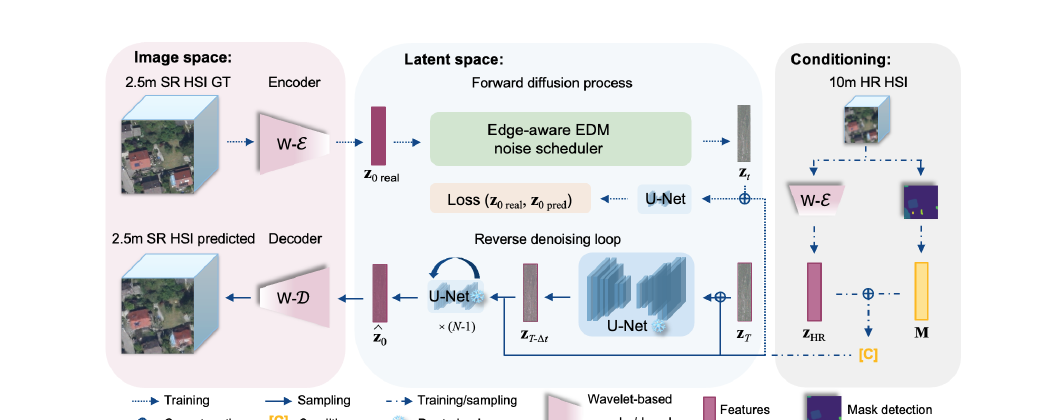
\includegraphics[width=\columnwidth]{fig/thesis/crops/gew_arch_clean-2.png}
\caption{GEWDiff RWA-PCA-EDM pipeline adapted from the primary paper~\cite{wang2026gew}.}
\label{fig:gewdiff-architecture}
\end{figure} It does not merge the published GEWDiff benchmark, locally reproduced WDC outputs, and CFG fine-tuning artifacts into one checkpoint-level claim. Those sources differ in dataset preparation, checkpoint state, and guidance-scale provenance.

\subsection{RWA-PCA Latent Representation}

Let $I_{LR}$ be the low-resolution hyperspectral image. At RWA level $j$, the transform produces main coefficients $V^j_{LR}$ and detail coefficients $w^j_{LR}$. Each detail coefficient is predicted by linear regression:

\begin{equation}
    \hat{w}^{j}_{i}=\beta^{j}_{i,0}+\sum_{k}\beta^{j}_{i,k}V^j_k,
\end{equation}

and the prediction residual is

\begin{equation}
    W^j_{LR}=w^j_{LR}-\hat{w}^{j}_{LR}.
\end{equation}

The encoder stores the final main coefficients $V^J_{LR}$ and the adjusted linear models $B_{LR}$, rather than storing the complete set of high-frequency coefficients for diffusion. PCA further transforms the main coefficients:

\begin{equation}
    (z_{LR},R_{LR})=\operatorname{PCA}(V^J_{LR}),
\end{equation}

where $z_{LR}$ is the compact latent input and $R_{LR}$ is retained for inverse PCA reconstruction. The reported implementation compresses the data to 20 PCA bands, balancing spectral information and diffusion cost.

After reverse diffusion predicts $\hat{z}_0$, inverse PCA recovers the predicted main coefficients and inverse RWA reconstructs the complete spectral image:

\begin{equation}
    \hat{V}^{J}_{SR}=\operatorname{I-PCA}(\hat{z}_0,R_{LR}),
\end{equation}

\begin{equation}
    \hat{I}_{SR}=\operatorname{I-RWA}(\hat{V}^{J}_{SR},B_{LR},W^j_{LR},J).
\end{equation}

RWA/PCA is therefore an input-to-latent and latent-to-output transform, not a separately trained end-to-end encoder-decoder~\cite{amrani2016rwa}. It reduces channel dimensionality and keeps the reverse process in a spectrally compact space. It cannot restore details absent from the low-resolution coefficient structure and remains dependent on accurate low-resolution geometric conditioning.

\subsection{EDM, Geometric Conditioning, and CFG}

GEWDiff uses Elucidating Diffusion Models (EDM)~\cite{karras2022edm} with continuous noise scale $\sigma$. Training noise is sampled by

\begin{equation}
    \sigma\sim\exp(\mathcal{N}(P_{mean}=-1.2,P_{std}=1.2)).
\end{equation}

The paper uses $t=-\log(\sigma_t)$ and reverse sampling with bounds $\sigma_{min}$ and $\sigma_{max}$. The schedule curvature $\rho$ controls the transition from higher to lower noise. The repository uses 50 sampling steps in CFG evaluations and the paper reports $\sigma_{max}=80$ and lower $\sigma_{min}$ values in the $0.02$--$0.2$ range as useful for preserving detail while limiting artifacts.

An edge-aware noise scheduler reduces perturbation around a binary edge map $E$:

\begin{equation}
    z_t=z_0+\sigma_t\epsilon\odot(1-E(1-\sigma_{norm})^{0.5}).
\end{equation}

Mask conditioning is additionally supplied to the denoiser, encouraging the reconstruction to preserve low-resolution structural boundaries. The training objective combines pixel reconstruction, perceptual loss, and gradient loss:

\begin{equation}
    L=\lambda(t)(0.8L_{pixel}+0.1L_{perc}+0.1L_{grad}).
\end{equation}

Pixel loss combines absolute or $L_2$ error with spectral angle, while perceptual and gradient terms emphasize semantic and spatial consistency.

Classifier-free guidance was later added to the implementation. During 10\% of training batches, the low-resolution image, mask, and edge tensors are replaced with zeros, creating an unconditional denoising route. Sampling blends conditional and unconditional predictions:

\begin{equation}
    \hat{z}_0=\hat{z}_{uncond}+w(\hat{z}_{cond}-\hat{z}_{uncond}),
\end{equation}

where $w=1$ gives the conditional prediction and $w>1$ strengthens the conditional direction relative to the unconditional prediction. This convention matches the locally documented CFG formulation. The repository contains CFG code and fine-tuning scripts, but exact guidance-scale labels and checkpoint provenance must be treated separately from the original GEWDiff training recipe.

\subsection{Published WDC Result}

The primary paper evaluates WDC after transfer from 8,000 training pairs and reports GEWDiff as better than the listed SNLSR baseline on the WDC test dataset. Table~\ref{tab:gew-published-wdc} reproduces the relevant PSNR, SSIM, SAM, CC, and RMSE values. These are published values with the paper's uncertainty reporting and are not a checkpoint-by-checkpoint reproduction.

\begin{table}[t]
\centering
\caption{Primary-paper WDC comparison.}
\label{tab:gew-published-wdc}
\small
\resizebox{\columnwidth}{!}{%
\begin{tabular}{lccccc}
\toprule
Method & PSNR $\uparrow$ & SSIM $\uparrow$ & SAM $\downarrow$ & CC $\uparrow$ & RMSE $\downarrow$ \\
\midrule
SNLSR & 35.734 & 0.7525 & 7.6613 & 0.7733 & 0.0471 \\
GEWDiff & 35.837 & 0.7747 & 7.4735 & 0.7906 & 0.0468 \\
\bottomrule
\end{tabular}}
\end{table}

The primary paper reports FID 238.12 for GEWDiff and 470.34 for SNLSR~\cite{wang2026gew}. Separately, the available local 28K CFG handover reports baseline FID 110.380661 and CFG FID 272.73706, versus 34.353846 and 35.327448 dB MPSNR respectively. FID is used as a relative perceptual statistic in an RGB feature space; it should not be combined directly with spectral metrics as if it measured the same physical error. The published WDC result establishes cross-dataset transfer in the paper, but does not prove that the later CFG modification retains the same test conditions.

\subsection{Verified CFG Guidance Sweep}

The repository contains a JSON aggregate for the \texttt{cfg\_step\_0022200.pth} checkpoint. It reports 50-step evaluations for guidance scales $1.0$, $1.5$, $2.0$, and $3.0$ on WDC.

\begin{table}[t]
\centering
\caption{Verified 22.2K checkpoint CFG sweep.}
\label{tab:gew-cfg-222k}
\small
\resizebox{\columnwidth}{!}{%
\begin{tabular}{lccccc}
\toprule
Scale & MPSNR $\uparrow$ & MSSIM $\uparrow$ & SAM $\downarrow$ & CC $\uparrow$ & RMSE $\downarrow$ \\
\midrule
1.0 & 35.283025 & 0.745424 & 8.310955 & 0.750282 & 0.048988 \\
1.5 & 35.197615 & 0.745700 & 8.023575 & 0.747466 & 0.049804 \\
2.0 & 34.869705 & 0.733240 & 8.286610 & 0.729033 & 0.051708 \\
3.0 & 34.543093 & 0.712087 & 9.269504 & 0.706650 & 0.054788 \\
\bottomrule
\end{tabular}}
\end{table}

At 22.2K, scale $1.0$ gives the highest MPSNR and lowest RMSE. Scale $1.5$ gives the lowest SAM in this sweep but also lowers MPSNR and CC. Scales $2.0$ and $3.0$ produce larger reconstruction losses. These results show that CFG does not monotonically improve every metric and that a stronger guidance scale is not necessarily better.

The repository also contains 31K metric directories, including values near 35.30 dB MPSNR. However, the individual metric files do not consistently record the associated guidance scale, and no complete 31K scale-index table reconstructs that association. Therefore, a claim such as \emph{31K checkpoint at scale 1.25} cannot be made from the available artifacts. Similarly, a 35.3105 dB value cannot be linked to a verified scale/checkpoint pair without additional run metadata.

\subsection{Engineering Constraints and Rationale for Pivot}

GEWDiff work included FSDP fine-tuning scripts, FP32, FP16, and BF16 investigations, Kaggle FSDP smoke tests, and checkpoint recovery experiments. Distributed fine-tuning required handling rank state, CPU-offloaded state dictionaries, streamed data, and checkpoint serialization. FP16-era training used legacy mixed-precision behavior, while later scripts and experiments explored BF16/FP32 and FSDP wrapping. These changes were part of an unstable engineering environment rather than controlled ablations of the diffusion architecture.

The computational bottleneck was also methodological. EDM sampling requires 50 reverse steps for the reported CFG evaluations; RWA/PCA compression, 3D U-Net denoising, repeated guidance sweeps, and FSDP communication increase memory and runtime. A complete multi-dataset experiment would require matched checkpoints, fixed guidance labels, and reproducible precision settings. These resources were not available with the required certainty in a single-workstation timeline.

The project therefore pivoted to SDANet, not because diffusion was shown to be universally weaker. The pivot selected a reconstruction model that can test region-specific attention with a 3.09M-parameter parameter-matched baseline and explicit ablations. GEWDiff remains a verified first direction: it demonstrates a credible generative HSI-SR architecture and identifies practical limits in conditioning, distributed training, and checkpoint reproducibility.

\section{Chapter 5: Proposed Methodology -- SDANet and SADS}
\label{sec:sads-method}

\subsection{Background and Motivation}

A hyperspectral image is represented as
$X \in \mathbb{R}^{C\times H\times W}$, where $C$ denotes the number of spectral bands and $H\times W$ denotes the spatial grid. Single-image HSI-SR seeks a mapping

\begin{equation}
    \hat{Y} = f_{\theta}(X_{LR}, X_{LMS}),
\end{equation}

where $X_{LR}$ is the low-resolution hyperspectral observation and $X_{LMS}$ is the bicubically upsampled LR-HSI used as a residual/skip branch. The mapping must improve spatial resolution without independently amplifying noise or introducing inter-band distortion.

The SDANet baseline combines convolutional feature extraction, dynamic spectral attention, frequency-domain feed-forward processing, and a PixelShuffle-based upsampler. Its core attention module, DSCA, estimates per-sample sparsity and then constrains each attention head to a learned number of entries. This design differs from fixed sparse attention: the sparsity level is data-dependent and can vary with the input. The implementation uses $n_{heads}=4$, feature dimension $n_{feats}=128$, and a default depth of two blocks in each of four stages.

DSCA is global in the following sense. Given a feature tensor
$X \in \mathbb{R}^{B\times D\times H\times W}$, depthwise convolutional projections produce query, key, and value tensors

\begin{equation}
    Q,K,V \in \mathbb{R}^{B\times N_h\times d_h\times HW},
\end{equation}

where $N_h$ is the number of heads and $d_h=D/N_h$ is the dimension per head. Normalized dot-product attention is

\begin{equation}
    A_{bhnm} = \frac{q_{bn h} \cdot k_{bm h}}{\sqrt{d_h}} \tau_h,
\end{equation}

where $\tau_h$ is a learned temperature and $h$ indexes attention heads. DSCA predicts one sparsity factor $s_b$ for each sample and uses it to define

\begin{equation}
    K_b = \left\lfloor 1 + (d_h-1)s_b \right\rfloor,
\end{equation}

with $1 \leq K_b \leq d_h$. Thus, a scene containing buildings, vegetation, water, roads, and shadowed areas receives the same regional attention capacity at the sparsity-budget level. This may be unnecessarily restrictive when feature statistics vary across spatial locations.

The regional extension therefore does not claim that all spatial attention operations must be independent. Instead, it identifies sparsity allocation as the first level at which spatial heterogeneity can be introduced with a small parameter change.

\subsection{Dynamic Spectral Channel Attention}

DSCA contains three coupled mechanisms:

\begin{enumerate}
    \item \textbf{A learned sparsity prediction path.} A depthwise $3\times3$ convolution followed by a pointwise multilayer gate predicts a channel gate map. Adaptive spatial pooling reduces this map to a scalar factor for the global baseline.

    \item \textbf{A hard--soft sparse mask.} Top-$k$ indices produce a hard binary mask. A continuous threshold computed from the mean and standard deviation of the attention scores produces a differentiable sigmoid mask. The straight-through estimate combines them:
    \begin{equation}
        M = M_{hard} + M_{soft} - \operatorname{detach}(M_{soft}).
    \end{equation}

    \item \textbf{A local--global residual branch.} The attention output is concatenated with a local depthwise-convolution branch and projected back to $D$ channels.
\end{enumerate}

For attention probabilities, $P = \operatorname{softmax}(A)\odot M$ is renormalized across the key dimension before multiplication by $V$. This construction preserves dense-valued attention in the forward pass at the mask level while allowing continuous gradients through the soft component.

\subsection{RegionalDSCA: $2\times2$ Spatial Partition}

SADS partitions each feature map into four quadrants:

\begin{equation}
\begin{aligned}
R_1 &= [0,H/2)\times[0,W/2), & R_2 &= [0,H/2)\times[W/2,W),\\
R_3 &= [H/2,H)\times[0,W/2), & R_4 &= [H/2,H)\times[W/2,W).
\end{aligned}
\end{equation}

The partition requires even spatial dimensions, and the network's reflection padding in \texttt{SDANET.forward\_origin} permits arbitrary input sizes by making $H$ and $W$ compatible with the downstream upsampling stages.

For region $g$, RegionalDSCA pools the learned gate map over its quadrant:

\begin{equation}
    s_g = \frac{1}{|R_g|}\sum_{(i,j)\in R_g} G_{:,i,j},
\end{equation}

where $G$ is the output of the gate projection. The factor is clipped to
$[\epsilon,1-\epsilon]$. Each region then receives

\begin{equation}
    K_g = \left\lfloor 1 + (d_h-1)s_g \right\rfloor.
\end{equation}

The implementation retains the baseline $Q$, $K$, and $V$ projections computed over the complete feature map. This choice keeps the global context available to every region and limits the modification to the sparsity-budget mechanism. Region $g$ selects values at flattened spatial indices

\begin{equation}
    I_g = \{iW+j:\; i,j\in R_g\},
\end{equation}

computes sparse attention using $K_g$, and reshapes the resulting tensor back to $(B,D,h_g,w_g)$. The four regional outputs are concatenated in top-left, top-right, bottom-left, bottom-right order before the local branch and output fusion.

\begin{figure}[t]
\centering
\resizebox{\columnwidth}{!}{%
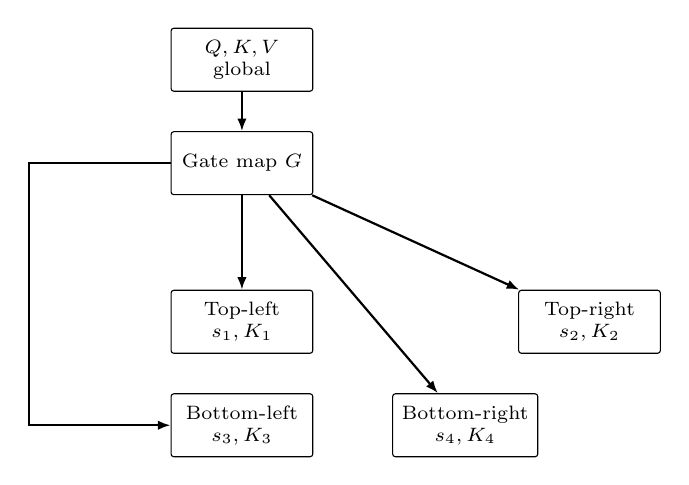
\begin{tikzpicture}[node distance=5mm,
box/.style={draw,rounded corners=1pt,minimum width=18mm,minimum height=8mm,align=center,font=\scriptsize},
arrow/.style={-{Latex[length=1.6mm]},thick}]
\node[box] (qkv) {$Q,K,V$\\global};
\node[box,below=5mm of qkv] (gate) {Gate map $G$};
\node[box,left=13mm of gate,below=12mm of gate] (tl) {Top-left\\$s_1,K_1$};
\node[box,right=26mm of tl] (tr) {Top-right\\$s_2,K_2$};
\node[box,below=5mm of tl] (bl) {Bottom-left\\$s_3,K_3$};
\node[box,right=10mm of bl] (br) {Bottom-right\\$s_4,K_4$};
\draw[arrow] (qkv) -- (gate);
\draw[arrow] (gate) -- (tl);
\draw[arrow] (gate) -- (tr);
\draw[arrow] (gate.west) -- ++(-18mm,0) |- (bl.west);
\draw[arrow] (gate) -- (br);
\end{tikzpicture}}
\caption{Code-accurate RegionalDSCA 2$\times$2 partition. Q/K/V are computed globally; only the top-$k$ budget is predicted independently for each quadrant.}
\label{fig:regional-dsca}
\end{figure}

This design can be interpreted as a modest hypothesis: spatial regions should influence the amount of attention sparsity, but the semantic affinity encoded by globally computed key and query tensors should remain shared.

\subsection{Fine-Gate Refinement}

The optional fine-gate variant adds a second $2\times2$ subdivision inside every coarse region. Therefore, it produces 16 spatial cells for feature maps divisible by four. A learned linear residual is initialized to zero:

\begin{equation}
    s_{g,c}^{\mathrm{fine}} = \operatorname{clamp}
    \left(s_g + w^{\top}\bar{G}_{g,c}+b,\epsilon,1-\epsilon\right).
\end{equation}

For the implementation used in the ablations, $\bar{G}_{g,c}$ is the spatial mean of the gate map over fine cell $(g,c)$. The fine-gate linear layer receives a vector of dimension $D$ and predicts a scalar residual. Both its weight and bias are initialized to zero, so the treatment model begins from the same coarse $2\times2$ sparsity map as the control model. This neutral initialization is important: it prevents the extra layer from changing the forward pass when the ablation begins, although it still adds trainable parameters and can change gradients after optimization.

The residual is intentionally local rather than a completely independent gate. It is connected to the same coarse factor $s_g$ and therefore cannot move arbitrarily far from the regional mean. This restriction can stabilize training by preserving the coarse spatial hierarchy, but it also limits content adaptation. For example, two fine cells in the same quadrant may receive opposite corrections even when the base factor is well matched, only if their pooled gate descriptors support a gradient through the learned linear layer.

The fine gate is enabled only in explicitly named treatment configurations. It is disabled in the standard SADS, RegionalFull, matched 66K, and independent-upsampler models unless a test or training option states otherwise. This implementation boundary makes it possible to compare the coarse regional mechanism and the additional fine residual separately.

\subsection{Network Integration and Upsampling}

The SADS block replaces the baseline fused-attention module with RegionalDSCA while preserving the remaining block structure:

\begin{equation}
X' = X + \operatorname{DropPath}(\operatorname{RegionalDSCA}(\operatorname{LN}(X))),
\end{equation}

\begin{equation}
X'' = X' + \operatorname{DropPath}(\operatorname{FEFFN}(\operatorname{LN}(X'))).
\end{equation}

The feed-forward network uses split real--imaginary frequency-domain filtering, together with $3\times3$ and $5\times5$ spatial branches. First, a pointwise expansion produces two feature halves. Two-dimensional FFT filtering is applied to each half through independently learned real and imaginary convolutions. The halves are then exchanged through a channel cross-interaction before inverse FFT reconstruction. Spatial $3\times3$ and $5\times5$ branches operate on the inverse-transformed values. This produces a mixed frequency--spatial residual that is projected back to the original feature width. Dropout and GELU activations are applied before projection, and the complete feed-forward residual is added to the attention residual.

Four residual stages each contain two SDA blocks in the default $[2,2,2,2]$ configuration. Every block uses layer normalization before attention and feed-forward branches, while drop-path probability increases linearly from zero to the stage limit of $0.4$. A $1\times1$ tail convolution creates a stage residual update. The complete body consists of four stage residuals followed by a convolutional tail. The baseline feature width is $128$, the number of heads is four, and each head has 32 dimensions. Consequently, DSCA selects between one and 32 channel/feature entries per attention head. The affinity matrix is $32\times32$ over channel dimensions, not a spatial key-position matrix.

The baseline upsampler is shared by its two $\times2$ stages and uses PixelShuffle in both stages, with a bicubic-interpolation branch available for fusion in some scale configurations. At $\times4$ resolution, the first PixelShuffle stage doubles the spatial dimensions and the second doubles them again. The independent-upsampler variant replaces this shared structure with two independent PixelShuffle stages, each with separate convolutional parameters. Its purpose is to separate uncertainty caused by the reconstruction head from uncertainty caused by regional attention. This variant is not parameter-neutral and is therefore reported only as an architectural diagnostic, not as a clean capacity-matched replacement.

A cropped SDANet architecture diagram is shown in Figure~\ref{fig:sdanet-architecture}. The network also preserves a bicubically upsampled low-resolution hyperspectral ($X_{LMS}$) processing branch. Its features are projected to the 128-channel width and cropped or combined with the upsampled residual at the target spatial size. The final $3\times3$ convolution produces 128 spectral bands. A reflection padding function makes the input height and width compatible with the fixed modular reconstruction pipeline before the final output is cropped back to the exact $\times 4$ dimensions.

\begin{figure}[!tbp]
\centering
\FloatBarrier
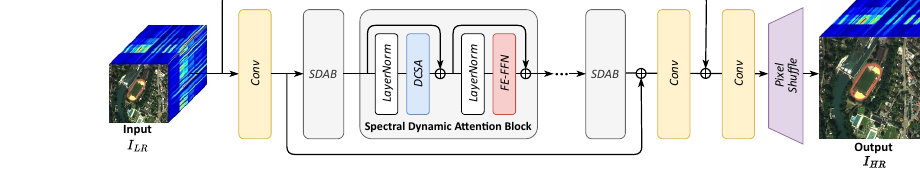
\includegraphics[width=\columnwidth]{fig/thesis/crops/sdanet_arch_final-2.png}
\caption{SDANet overall framework and DSCA detail adapted from the local preprint~\cite{wang2026sdanet}.}
\label{fig:sdanet-architecture}
\end{figure}

\subsection{Controlled Ablation Scope}

The implementation supports the following comparisons:

\begin{itemize}
    \item \textbf{Global baseline:} original DSCA with one sparsity factor per sample.
    \item \textbf{Regional SADS:} independent sparsity factors over a $2\times2$ grid.
    \item \textbf{Fine-gate control:} $2\times2$ regional factors with the residual fine gate disabled.
    \item \textbf{Fine-gate treatment:} the same configuration with the residual fine gate enabled.
    \item \textbf{Independent upsampler:} two independently parameterized $\times2$ PixelShuffle stages, tested from a fine-tuned and a scratch initialization.
    \item \textbf{Matched-budget continuation:} regional training continued to the same 66K iteration budget as the independent comparison where available.
\end{itemize}

The report does not treat all of these runs as independent evidence of a method ranking. Configurations, checkpoints, and iteration budgets must be compared only within explicitly matched protocols. Historical \texttt{RegionalFull} evaluations and matched 66K evaluations, for example, use different comparison definitions and must remain separate.

\subsection{Scope and Limitations}

The initial evidence is concentrated on Chikusei and is intended to test whether region-dependent sparsity allocation changes reconstruction behavior. A fixed $2\times2$ grid cannot adapt to content boundaries and may split a single material into multiple regions. The gate itself is inferred from the feature map, so it does not receive a direct supervised spatial-region label. Any gain must therefore be validated by spectral and spatial diagnostics rather than attributed to regional partitioning alone.

The current ablation setup is not sufficient to establish cross-dataset or cross-sensor generalization. Conclusions are limited to the evaluated checkpoint, scene, split, degradation protocol, and tile set. Pavia or other datasets are included in future experimental plans only when the corresponding data pipeline, split, and evaluation results are completed and verified.

\section{Chapter 6: Experimental Setup and SDANet/SADS Results}
\label{sec:sads-results}

\subsection{Dataset and Degradation Protocol}

The experiments use Chikusei hyperspectral data~\cite{yokoya2016chikusei}, organized into a spatially separated train, validation, and test protocol. The low-resolution input and its $X_{LMS}$ bicubic-upsampled companion are constructed for $\times4$ super-resolution. Training samples are $128\times128$ ground-truth patches augmented by horizontal flipping and rotation. The training configuration uses Adam with learning rate $10^{-4}$, weight decay zero, and $(\beta_1,\beta_2)=(0.9,0.99)$. The main loss is L1 with a spectral angle loss of weight $0.2$. Training state was refreshed by EMA, and the reported checkpoints use the EMA parameter key \texttt{params\_ema}.

The held-out test set contains four $512\times512\times128$ spatial tiles extracted from one Chikusei scene. The configured split contains 651 training records and 62 validation records; all principal SDANet runs use one NVIDIA RTX 4000 Ada GPU, batch size 16, manual seed 10, Adam at learning rate $10^{-4}$, EMA decay $0.999$, and L1 plus spectral-angle losses. The aggregate test result is the arithmetic mean of four tile-level values. It is therefore more accurately described as the mean over four test tiles, not as evidence obtained from four independent scenes or independent data acquisitions. Per-tile metric variation is reported with the arithmetic mean to expose this distinction.

The training and evaluation split must also be distinguished from validation fusion diagnosis and exploratory test-set fusion. Training patches and validation patches are held out from the four test tiles, but the validation split was used to tune and compare ablation hypotheses during development. Results selected by visualizing or optimizing on validation patches are diagnostic; they are not unbiased test results. The 62 validation samples used in the fusion analysis are overlapping $128\times128$ patches on a buffered spatial grid. Adjacent patches can share large image regions, so their metrics are correlated even though 62 numerical records are reported. This is why the fusion section uses descriptive means and never claims a formal significance test.

The bicubic degradation also matters. It is a controlled synthetic $\times4$ setting that provides exact ground truth and stable metric calculation. It does not establish robustness to real sensor noise, atmospheric effects, registration errors, or unknown blur kernels. Any future extension to real-world HSI-SR should therefore include the degradation process explicitly rather than treating bicubic low-resolution construction as a universal measurement model.

Evaluation was performed with PyTorch 2.11.0 and CUDA 12.8. Deterministic-oriented settings included CUDA cuBLAS workspace configuration and deterministic algorithms, while TF32 and cuDNN benchmarking were disabled. These settings reduce run-to-run variability, but they do not guarantee bitwise reproducibility across unrelated hardware and software stacks.

\subsection{Evaluation Metrics}

Let $Y$ and $\hat{Y}$ denote the reference and reconstructed hyperspectral tensors. The implementation reports the following metrics:

\begin{itemize}
    \item \textbf{MPSNR:} mean peak signal-to-noise ratio across the evaluated bands. It is a spatial--spectral fidelity index in which higher values indicate lower reconstruction error.
    \item \textbf{SSIM:} structural similarity~\cite{wang2004ssim} averaged over the scene-level or tile-level evaluation. Higher values indicate better structural agreement.
    \item \textbf{SAM:} spectral angle mapper~\cite{yuhas1992sam}, defined for a pixel pair $y,\hat{y}$ as
    \begin{equation}
        \operatorname{SAM}(y,\hat{y}) = \cos^{-1}\left(
        \frac{y^{\top}\hat{y}}{\|y\|_2\|\hat{y}\|_2+\epsilon}
        \right).
    \end{equation}
    It is reported in degrees and lower values indicate better spectral preservation.
    \item \textbf{ERGAS:} a scale-sensitive multi-band reconstruction error index~\cite{wald2002ergas} in which lower values indicate better performance.
    \item \textbf{CC:} correlation coefficient between reference and reconstruction. Higher values indicate stronger correlation.
\end{itemize}

MSE and MAE are additionally used in spatial and validation diagnostics. No metric should be interpreted independently: MPSNR may improve while a spectral index regresses, or spatial improvement may be concentrated in only a subset of the test tiles.

\subsection{Matched 66K Budget Comparison}

The primary controlled comparison compares global SDANet and regional SADS after continuation to the same 66K iteration checkpoint. The global and regional checkpoints contain $3{,}086{,}272$ parameters, and both use the EMA parameters at 66K iterations. The test aggregation is arithmetic over the same four spatial tiles.

\begin{table}[t]
\centering
\caption{Matched 66K comparison on four Chikusei test tiles. Differences are descriptive and not evidence of statistical significance.}
\label{tab:matched66k}
\small
\resizebox{\columnwidth}{!}{%
\begin{tabular}{lccccc}
\toprule
Method & SSIM $\uparrow$ & MPSNR $\uparrow$ & SAM $\downarrow$ & ERGAS $\downarrow$ & CC $\uparrow$ \\
\midrule
Global SDANet & 0.944014 & 40.314650 & 2.311066 & 4.966979 & 0.956202 \\
Regional SADS & 0.943984 & 40.313355 & 2.311717 & 4.967364 & 0.956176 \\
\bottomrule
\end{tabular}}

\end{table}

At this budget, regional SADS is slightly lower than the global baseline.\footnote{The 40.313355 dB Regional SADS value is from the matched 66K EMA-checkpoint comparison in \texttt{Matched66K\_Analysis/summary.json}. The 40.314303 dB RegionalFull value is an independent final-reproduction evaluation in \texttt{results/final\_repro/SDANetRegionalFull\_Chikusei\_x4\_test}; it uses a different checkpoint/training path and is not a re-evaluation of the matched 66K pair. The 0.000948 dB rounding-level difference is therefore retained as a checkpoint-provenance distinction.} The differences are $-0.001295$ dB in MPSNR, $+0.000651^\circ$ in SAM, $+0.000385$ in ERGAS, $-0.000031$ in SSIM, and $-0.000026$ in CC. Regional MSE and MAE are also slightly larger in the aggregate. These differences are small relative to scene-level variation and do not establish a reproducible regional advantage.

The matched comparison also allows an important negative conclusion. The 66K comparison does not validate the claim that regional sparsity alone consistently improves reconstruction. It instead shows that a parameter-matched spatial partition can perform approximately as well as a global budget, while preserving the spatial diagnostic capacity to identify tile- and window-level trade-offs.

\subsection{Spatial and Spectral Diagnostics}

The matched outputs were analyzed on a per-pixel, per-band basis. The spectral-band results are mixed. In the post-hoc 19--27 range, Regional SADS has lower aggregate RMSE on all 9 bands (mean improvement 0.0186\%). Across all 128 bands, Regional is lower on 32 and Global on 96; in the separate 80--93 range, Global is lower on all 14 bands. These exploratory patterns do not support uniform regional superiority.

Regional and global mean pixel RMSE values are nearly identical, but the result is not spatially uniform. Across the four tiles, regional RMSE is lower only for tile 1 (0.007926 versus 0.007930); it is higher for tiles 0, 2, and 3. Across 900 overlapping $64\times64$ windows, regional MSE is lower in 389 windows and global MSE is lower in 511 windows. This pattern indicates that regional benefit is concentrated in local areas rather than consistently distributed across the scene.

A separate quadrant analysis uses the four spatial quadrants within each test tile. Regional MSE is lower in 5 of 16 quadrants and higher in 11. The strongest regional window has 11.758\% lower MSE, while selected global-favouring windows show approximately $5$--$10\%$ lower global MSE. These local effects are descriptive; the selected regions were not randomly sampled and were not used for model selection.

\begin{figure*}[t]
\centering
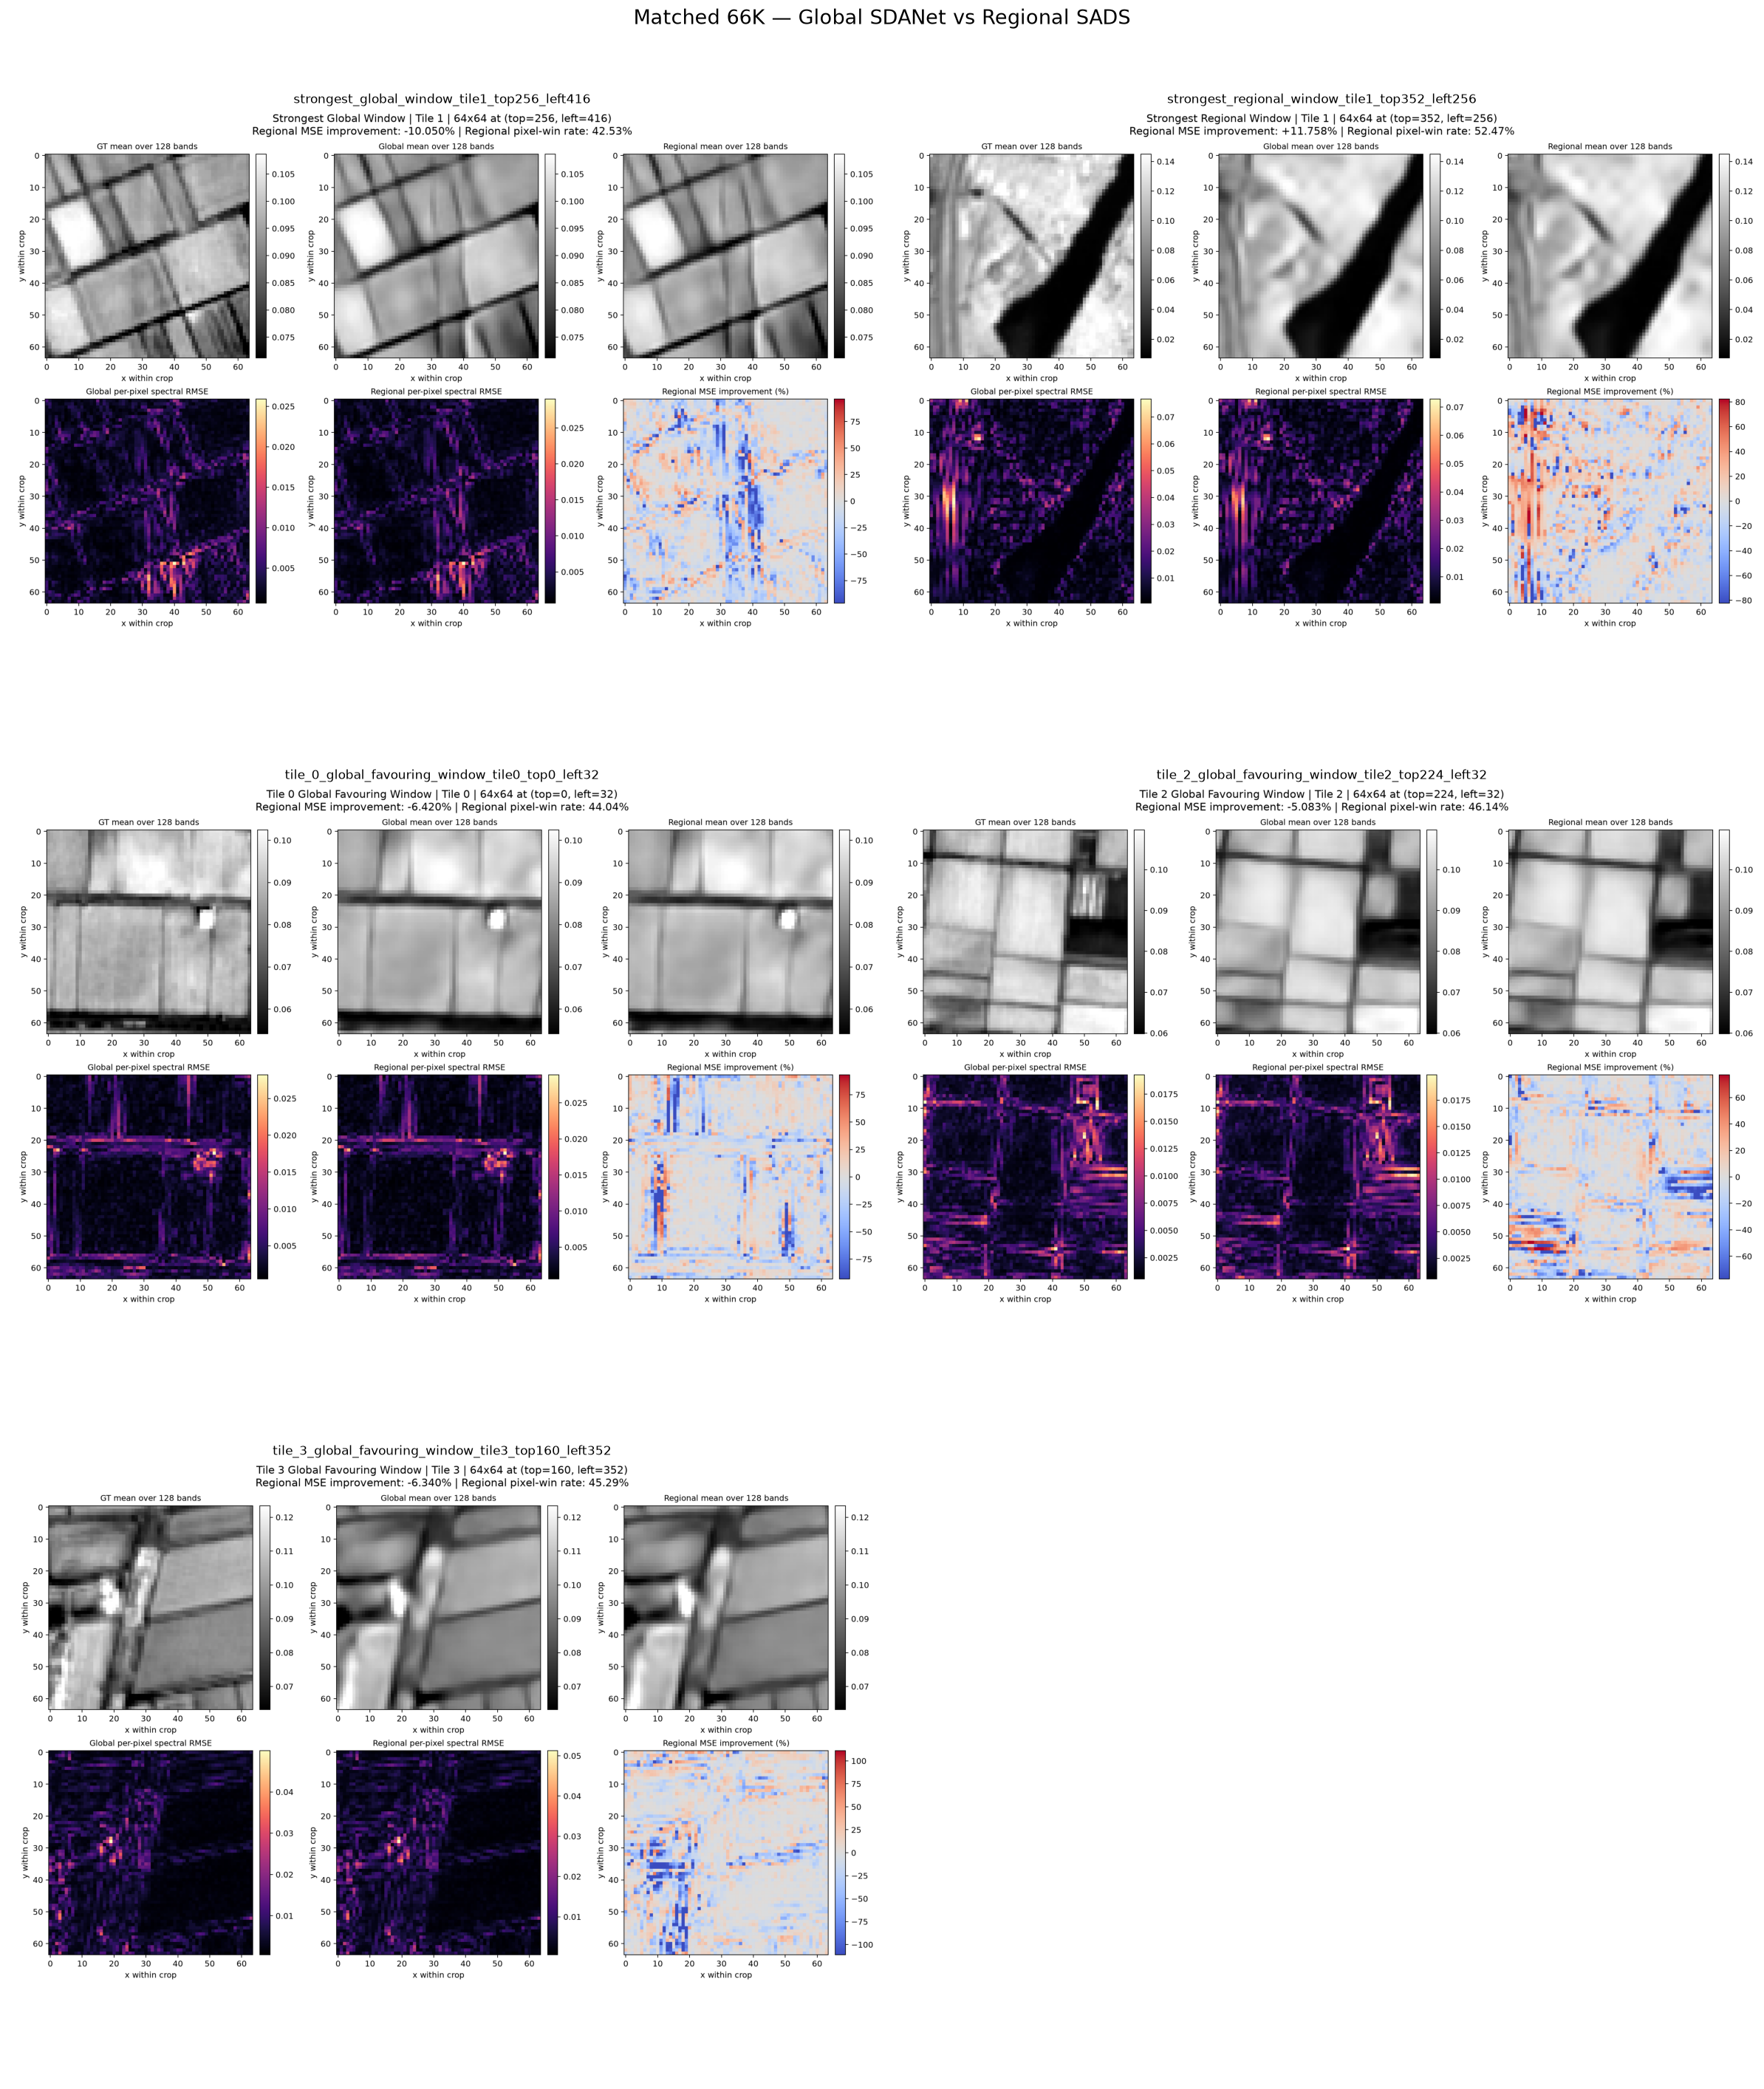
\includegraphics[width=0.95\textwidth]{../../results/Matched66K_Analysis/qualitative_regions/qualitative_contact_sheet.png}
\caption{Matched 66K qualitative regions. Averaged bands show spatial context; the second row reports per-pixel spectral RMSE and relative Regional-vs-Global MSE improvement. Selected regions are illustrative, not random or confirmatory samples.}
\label{fig:matched-qualitative}
\end{figure*}

\begin{figure*}[t]
\centering
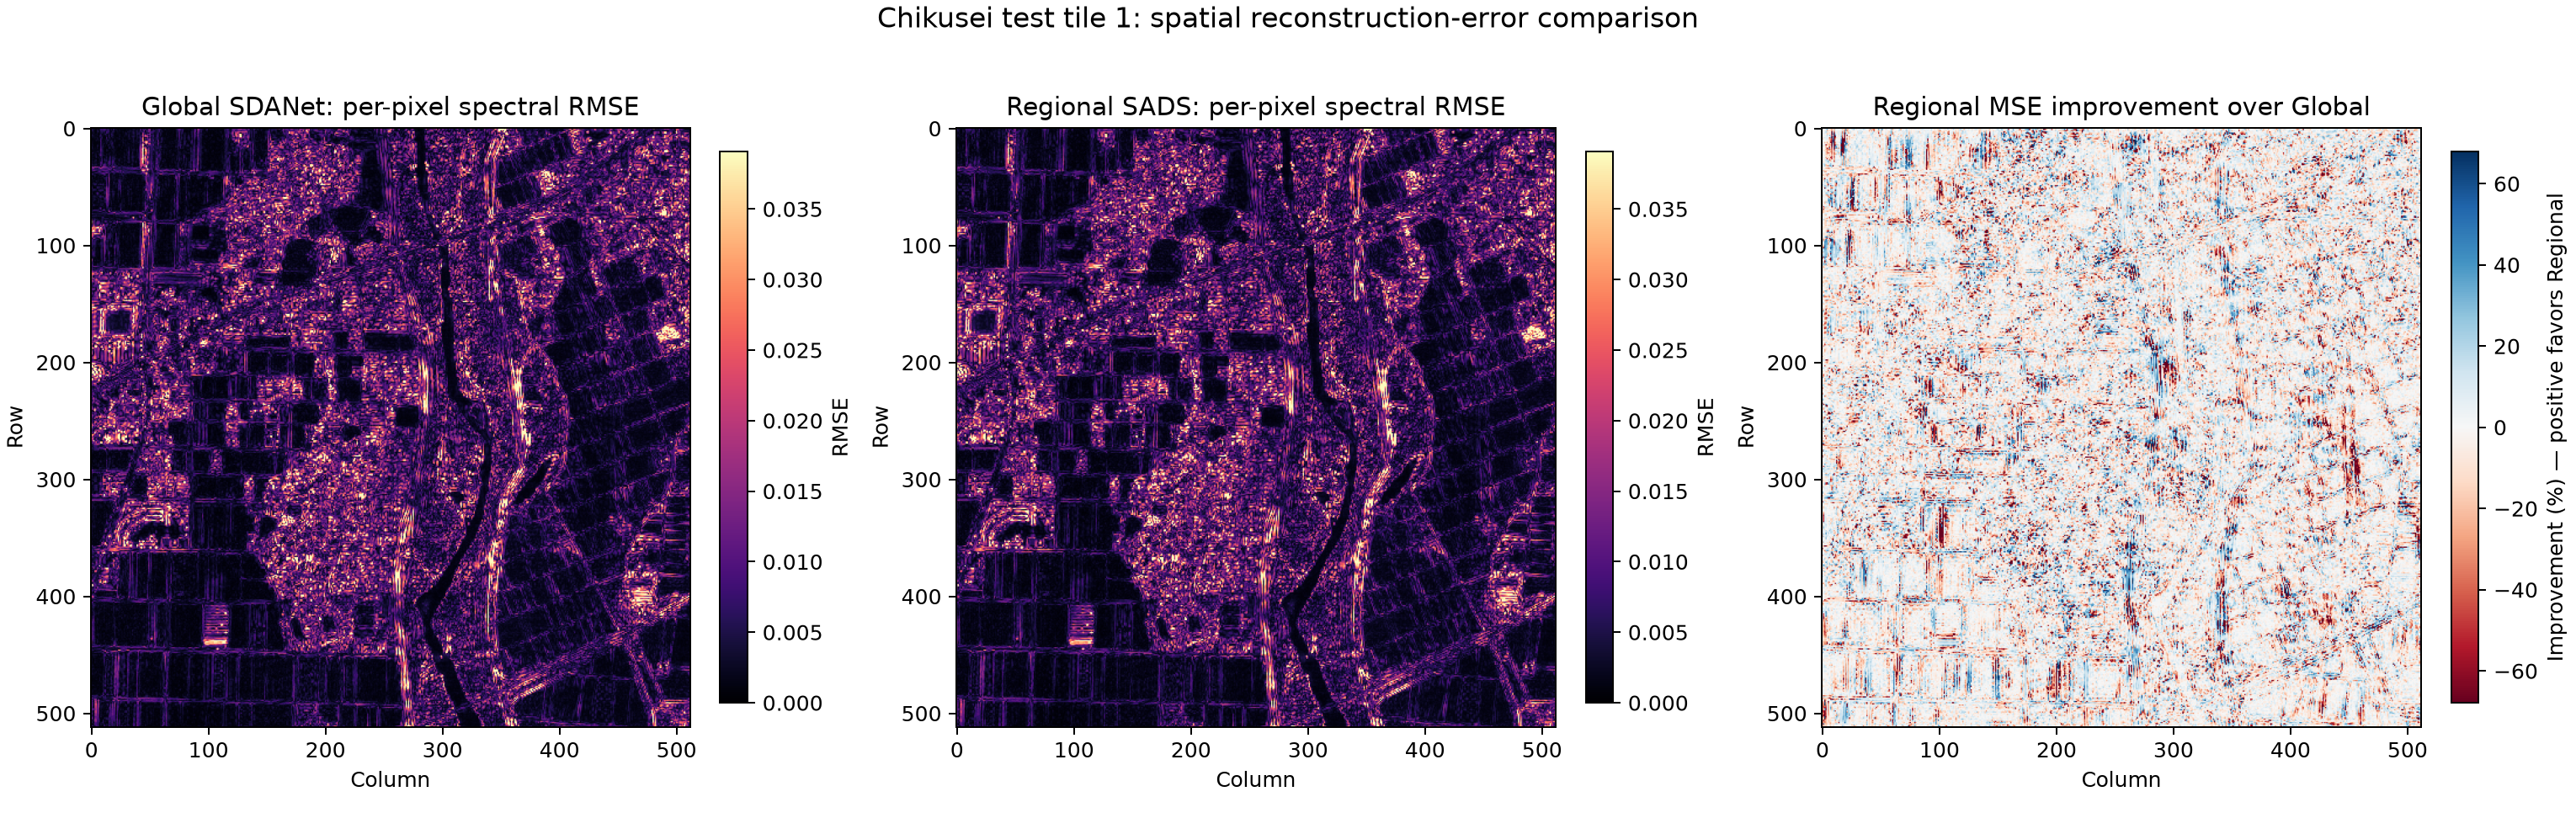
\includegraphics[width=0.90\textwidth]{../../results/Matched66K_Analysis/spatial_spectral/tile_1_spatial_error_maps.png}
\caption{Matched 66K Global-vs-Regional spatial error maps for Chikusei test tile 1, a regional RMSE-favouring tile in the aggregate diagnostic.}
\label{fig:matched-error-maps}
\end{figure*}

\subsection{Fine-Gate 5K Control and Treatment}

A 5K continuation experiment separates the effect of enabling the optional fine gate from all other architectural choices. The control uses RegionalDSCA with fine gating disabled. The treatment uses the same initialization and 5K continuation with the residual fine gate enabled. Both retain the four-regional architecture and the longer RegionalFull checkpoint is not an equivalent matched baseline for this pair.

\begin{table}[t]
\caption{Checkpoint-context results on four Chikusei test tiles. The fine-gate control and treatment form the matched 5K continuation pair; the 33K and 66K reference checkpoints have different training budgets and are not matched comparisons.}
\label{tab:finegate}
\small
\resizebox{\columnwidth}{!}{%
\begin{tabular}{lccccc}
\toprule
Checkpoint & SSIM $\uparrow$ & MPSNR $\uparrow$ & SAM $\downarrow$ & ERGAS $\downarrow$ & CC $\uparrow$ \\
\midrule
Global SDANet (33K) & 0.940856 & 40.031740 & 2.403565 & 5.165315 & 0.953247 \\
RegionalFull (66K) & 0.943984 & 40.314303 & 2.311431 & 4.966427 & 0.956183 \\
Fine-gate Control (66K+5K) & 0.944033 & 40.317727 & 2.309830 & 4.965020 & 0.956218 \\
Fine-gate Treatment (66K+5K) & 0.944067 & 40.321820 & 2.309864 & 4.962553 & 0.956257 \\
\bottomrule
\end{tabular}}

\end{table}

Enabling the fine gate improves MPSNR by $0.004093$ dB, ERGAS by $0.002468$, SSIM by $0.000034$, and CC by $0.000039$. SAM increases by $0.000034^\circ$. Thus, the treatment is associated with a small spatial and aggregate fidelity improvement but does not reduce spectral angle in this run. The effect is too small and the sample set too limited to claim a stable fine-gate benefit. This was a four-tile, single-scene comparison, and the reported change is not evidence of statistical significance.

The first two rows are historical reference checkpoints with different training budgets; differences combine architecture and training duration and must not be attributed to regional sparsity alone. The final two rows are the paired fine-gate continuation evaluated from the same 66K initialization.

\subsection{Independent Upsampler and Fusion Diagnostics}

The independent-upsampler variant has $3{,}676{,}608$ parameters, compared with $3{,}086{,}272$ parameters in the regional and global standard models. It therefore should not be interpreted as a parameter-neutral ablation. On 62 overlapping validation patches, RegionalFull achieves mean MPSNR 41.648806 dB, SAM 2.180580$^\circ$, ERGAS 4.420482, SSIM 0.949552, and CC 0.947458. The independent upsampler obtains MPSNR 41.385334 dB, SAM 2.252128$^\circ$, ERGAS 4.581597, SSIM 0.946888, and CC 0.944278. The regional model therefore leads on this validation diagnostic, but the patches overlap spatially and the metric is not an independent generalization estimate.

A scalar output blend was evaluated on the validation split:
\begin{equation}
    \hat{Y}_{\alpha}=\alpha\hat{Y}_{Regional}+(1-\alpha)\hat{Y}_{Independent},
\end{equation}
with $\alpha \in [0.5,1.0]$. The alpha sweep was not a learned output gating mechanism. The best fixed validation mean MPSNR occurs near $\alpha=0.80$: 41.664855 dB, with SSIM 0.949691, SAM 2.172502$^\circ$, ERGAS 4.416337, and CC 0.947644. A learned dynamic regional gate reports MPSNR 41.655475 dB and SSIM 0.949617, below the best fixed-alpha MPSNR but above the independent-upsampler baseline.

The fixed blend and dynamic gate were subsequently evaluated on the same held-out four-tile Chikusei test split. This is an exploratory ablation on the fixed 4-tile split, not blind cross-scene or cross-dataset validation. The dynamic gate also uses ground-truth-derived validation metrics only for diagnosis; the gate does not receive ground truth during forward inference.

\begin{table}[t]
\caption{Exploratory test-set fusion comparison on the four Chikusei test tiles.}
\label{tab:test-fusion}
\centering
\small
\resizebox{\columnwidth}{!}{%
\begin{tabular}{lccccc}
\toprule
Method & SSIM $\uparrow$ & MPSNR $\uparrow$ & SAM $\downarrow$ & ERGAS $\downarrow$ & CC $\uparrow$ \\
\midrule
Regional Full & 0.943984 & 40.314303 & 2.311431 & 4.966427 & 0.956183 \\
Independent Upsampler & 0.941506 & 40.091744 & 2.375062 & 5.122399 & 0.953870 \\
Fixed $\alpha=0.8$ & 0.944295 & 40.346249 & 2.300718 & 4.950650 & 0.956470 \\
Dynamic Regional Gate & 0.944089 & 40.324359 & 2.307988 & 4.961067 & 0.956277 \\
\bottomrule
\end{tabular}}
\end{table}

\begin{figure*}[t]
\centering
\includegraphics[width=0.82\textwidth]{../../results/final_repro/visualizations/scene_1_qualitative_comparison.png}
\caption{Chikusei test-tile qualitative comparison. Local reconstruction and error panels are shown for visual context; error maps for the ground-truth reference are zero by construction. The panel is not an unbiased statistical comparison.}
\label{fig:chikusei-qualitative}
\end{figure*}

On the test tiles, the dynamic gate weights remained high, ranging from $0.961067$ to $0.989010$ across quadrants and tiles. Thus the gate retained a strong regional-reconstruction bias rather than selecting the independent upsampler uniformly. The validation-selected fixed $\alpha=0.8$ blend gave the highest test MPSNR and SSIM and the lowest SAM and ERGAS, but this split-to-split transfer does not demonstrate blind generalization.

\subsection{Discussion and Interpretation}

The evidence supports four limited conclusions. First, region-dependent sparsity is implementable within the SDANet parameter budget and preserves nearly the same matched-checkpoint performance as global sparsity. This is meaningful because the regional and global checkpoints have identical parameter counts and are evaluated after 66K iterations. It demonstrates that the spatial modification does not create a simple capacity advantage.

Second, the regional benefit is uneven at both spatial and spectral scales. The aggregate MPSNR difference is much smaller than scene-level variation, while some sliding windows show a stronger regional or global advantage. The result is therefore mechanistically informative but not uniformly positive. It should not be summarized as either a clear win or a clear failure of regional attention.

Third, the fine-gate treatment is a small paired modification rather than a broad architectural redesign. Its near-zero initialization makes the control and treatment forward paths equivalent at the first fine-gate step, while 5K iterations allow residual coefficients to adapt. The resulting 0.004093 dB MPSNR change is too small to justify a strong claim, even though the paired protocol improves confidence relative to comparisons with unrelated checkpoints.

Fourth, the independent-upsampler and fusion analyses show that the output reconstruction head is an important complement to attention design. The fixed $\alpha=0.80$ blend outperforms the individual validation baselines on multiple mean metrics, but the alpha was chosen from the same validation split and the 62 patch records are correlated. It is evidence of predictive complementarity, not held-out generalization.

The validation and test fusion results are complementary: the validation sweep identifies fixed $\alpha=0.80$ as a useful local design diagnostic, while the test-table results quantify the same fixed model combination and the learned gate on the four-tile split. Neither result establishes generalization outside Chikusei.

The report must avoid a compound interpretation that regional attention, fine gating, independent upsampling, and fusion are mutually additive. They were not evaluated as one fully orthogonal factor experiment. The independent-upsampler model has more parameters, the fine-gate comparison has 5K checkpoints, the matched comparison has 66K checkpoints, and the fusion analysis uses validation and fixed test-split prediction combinations. Mixing these protocols into a single ranking would overstate certainty.

\FloatBarrier
Several claims remain unsupported. It is not established that SADS dominates SDANet, that the $2\times2$ grid is optimal, or that fine-gate and fusion variants transfer to Pavia or another sensor. It is likewise inappropriate to compare every run as a single ordered leaderboard, because the checkpoints differ in iteration count, parameter count, and model family. A defensible interpretation of the work is that spatial partitioning offers a useful mechanism for allocating spectral attention sparsity, while its net benefit depends on checkpoint and region selection.

\FloatBarrier
\section{Chapter 7: Conclusion and Future Work}
\label{sec:conclusion}

\subsection{Unified Two-Semester Summary}

This thesis traces a two-semester progression through hyperspectral image super-resolution, beginning with baseline reconstruction engineering and ending with controlled regional attention diagnostics. Semester-1 work established a reproducible HSI-SR data and metric pipeline through SSRNet, HSRnet, MSHSR, and CAVE/Harvard/Chikusei-oriented experiments. It also demonstrated the importance of data shape, band order, padding, checkpoint identity, and metric registration before architectural conclusions could be made.

Semester-2 began with GEWDiff as a generative reconstruction candidate. The method combines RWA and PCA to compress the hyperspectral input, EDM to model the reverse noise process, mask and edge conditioning to preserve geometry, and pixel/perceptual/gradient losses to stabilize fidelity. The primary GEWDiff paper reports strong WDC transfer. Local CFG implementation and 22.2K results show that guidance $1.0$ gives the best MPSNR and RMSE in the verified sweep, while scale $1.5$ improves SAM and stronger scales degrade the reconstruction. FSDP, precision, and checkpoint recovery work also established that reproducible distributed diffusion experiments require matched execution metadata. The available 28K handover also showed MPSNR improve from 34.353846 dB to 35.327448 dB, while FID deteriorated from 110.380661 to 272.73706. This was a mixed reconstruction-versus-perceptual outcome, not an overall CFG improvement. The 28K handover is kept separate from the verified 22.2K guidance sweep because its checkpoint and guidance provenance differ.

The project then moved to SDANet as a parameter-matched reconstruction baseline. The baseline uses a 3.09M-parameter dynamic spectral channel attention module with a learned top-$k$ sparsity factor. The RegionalDSCA/SADS variant assigns independent factors to four spatial quadrants while retaining globally computed Q/K/V affinity and the remaining SDANet block structure.

\subsection{Principal Findings}

The matched 66K comparison produced nearly identical global and regional results on four Chikusei test tiles. Regional SADS was 0.001295 dB lower in MPSNR and showed slightly worse SAM, ERGAS, SSIM, and CC. It is not correct to describe this result as a universal SADS improvement. It instead demonstrates that a parameter-matched regional mechanism can preserve baseline performance while providing local spatial control.

The spatial diagnostics reveal mixed behavior. Tile 1 showed a small regional RMSE improvement, while tiles 0, 2, and 3 showed regional RMSE regressions. Regional MSE was lower in 5 of 16 quadrants and in 389 of 900 sliding windows. Band-range behavior was uneven as well. These findings explain why aggregate MPSNR and SSIM can remain nearly unchanged despite a spatially variable mechanism.

The 5K fine-gate paired experiment on four test tiles from one Chikusei scene produced only a 0.004093 dB MPSNR improvement and a $0.002468$ ERGAS improvement in favor of the treatment, while SAM increased slightly. This is not sufficient evidence for a stable or large fine-gate benefit. Independent-upsampler and fixed/dynamic-fusion experiments show predictive complementarity between reconstruction heads on both the validation diagnostic and the exploratory 4-tile Chikusei test split. These results are neither held-out cross-dataset generalization nor statistically significant evidence and should not be combined into an orthogonal component ranking.

\subsection{Limitations}

The evidence is limited to one hyperspectral scene, synthetic $\times4$ degradation, and four spatial test tiles. The test tiles are not independent scenes, and the 62 validation fusion patches overlap spatially. Aggregate differences are descriptive rather than statistical significance estimates. No Pavia, M2, OCTTA, or real-sensor result is included because the corresponding verified pipelines and results are unavailable.

The $2\times2$ partition is fixed and cannot follow boundaries in the image. It may divide a natural material across regions or group unrelated materials inside one quadrant. The gate is learned from feature statistics and is not supervised with semantic region labels. The fine-gate, upsampler, and fusion variants differ in parameter count or training budget, so their effects cannot be isolated by simply comparing final metrics.

GEWDiff evidence is also bounded. Published WDC results establish the primary paper's benchmark, but they are not a direct reproduction of every local CFG checkpoint. The 22.2K CFG sweep is verified, while the 31K guidance-scale mapping and 35.3105 dB value are not supported by complete run metadata. FSDP and precision experiments should not be interpreted as controlled ablations of the diffusion architecture.

\subsection{Future Work}

Future SADS work should use content-aware or multi-scale spatial partitions rather than a fixed grid. Learned boundary-aware grouping, deformable region assignments, and validation on multiple independent scenes would test whether regional sparsity can generalize beyond Chikusei. A parameter-matched and seed-repeated experiment should also separate checkpoint variance from model variance.

Future GEWDiff work should retain the scale, checkpoint, precision, sampler, and dataset manifest with every run. Guidance sweeps should use a held-out test set and report uncertainty over repeated checkpoints or seeds. RWA/PCA compression should be compared under fixed sampling steps and fixed hardware for a fair efficiency analysis.

A final unified study could evaluate GEWDiff and SDANet under the same degradation, dataset, split, and metric protocol. This comparison would test whether generative diffusion and reconstruction attention complement each other rather than merely reproducing separate historical benchmarks. It would also clarify whether a reconstruction model, a diffusion model, or a controlled fusion offers the best trade-off among fidelity, runtime, memory, and spectral stability.

\FloatBarrier
\addcontentsline{toc}{section}{References}
\begin{thebibliography}{99}
\bibitem{wang2020ssrnet} Q. Wang, Q. Li, and X. Li, ``Spatial-Spectral Residual Network for Hyperspectral Image Super-Resolution,'' arXiv:2001.04609, 2020.
\bibitem{wang2026gew} S. Wang, J. He, N. Blasco Andreo, and X. X. Zhu, ``GEWDiff: Geometric Enhanced Wavelet-based Diffusion Model for Hyperspectral Image Super-resolution,'' in \textit{Proc. AAAI Conf. Artificial Intelligence}, vol. 40, no. 12, pp. 10109--10117, 2026, doi: 10.1609/aaai.v40i12.37978.
\bibitem{wang2026sdanet} T. Zhang, F. Gao, L. Qi, J. Dong, and Q. Du, ``Spectral Dynamic Attention Network for Hyperspectral Image Super-Resolution,'' \textit{IEEE Geoscience and Remote Sensing Letters}, vol. 23, 2026, art. no. 5504005, doi: 10.1109/LGRS.2026.3689855.
\bibitem{hu2022hsrnet} J.-F. Hu, T.-Z. Huang, L.-J. Deng, T.-X. Jiang, G. Vivone, and J. Chanussot, ``Hyperspectral Image Super-Resolution via Deep Spatiospectral Attention Convolutional Neural Networks,'' \textit{IEEE Trans. Neural Networks and Learning Systems}, vol. 33, no. 12, pp. 7251--7265, Dec. 2022.
\bibitem{zhang2025mshsr} J. Zhang, H. Qu, J. Jia, Y. Li, B. Jiang, X. Chen, and J. Peng, ``Multiscale Spatial--Spectral CNN--Transformer Network for Hyperspectral Image Super-Resolution,'' \textit{IEEE Journal of Selected Topics in Applied Earth Observations and Remote Sensing}, vol. 18, pp. 12116--12132, 2025.
\bibitem{wang2023survey} X. Y. Wang, Q. Hu, Y. S. Cheng, and J. Y. Ma, ``Hyperspectral Image Super-Resolution Meets Deep Learning: A Survey and Perspective,'' \textit{IEEE/CAA Journal of Automatica Sinica}, vol. 10, no. 8, pp. 1668--1691, Aug. 2023.
\bibitem{karras2022edm} T. Karras, M. Aittala, T. Aila, and S. Laine, ``Elucidating the Design Space of Diffusion-Based Generative Models,'' Advances in Neural Information Processing Systems, 2022.
\bibitem{amrani2016rwa} N. Amrani, J. Serra-Sagrista, V. Laparra, M. W. Marcellin, and J. Malo, ``Regression Wavelet Analysis for Lossless Coding of Remote-Sensing Data,'' \textit{IEEE Trans. Geoscience and Remote Sensing}, vol. 54, no. 9, pp. 5616--5627, 2016.
\bibitem{yuhas1992sam} R. H. Yuhas, A. F. H. Goetz, and J. W. Boardman, ``Discrimination among Semi-Arid Landscape Endmembers Using the Spectral Angle Mapper,'' JPL Summaries, 1992.
\bibitem{yokoya2016chikusei} N. Yokoya and A. Iwasaki, ``Airborne Hyperspectral Data over Chikusei,'' Space Application Laboratory, University of Tokyo, Japan, Tech. Rep. SAL-2016-05-27, May 2016.
\bibitem{wang2004ssim} Z. Wang, A. C. Bovik, H. R. Sheikh, and E. P. Simoncelli, ``Image Quality Assessment: From Error Visibility to Structural Similarity,'' \textit{IEEE Trans. Image Processing}, vol. 13, no. 4, pp. 600--612, Apr. 2004.
\bibitem{wald2002ergas} G. Wald, \textit{Data Fusion: Definitions and Architectures: Fusion of Images of Different Spatial Resolution}, Les Presses du Minitec, 2002.
\end{thebibliography}

\end{document}
